% =====================================================================
% ejercicio07.tex
% Responsabilidad única: comparar el efecto de estandarizar las
% variables sobre un mismo modelo KNN (k=5), y justificar la elección
% de modelo con base en las métricas obtenidas.
% =====================================================================
\subsection{Ejercicio 7 --- KNN con $k=5$: sin escalar vs. estandarizado}

\begin{table}[H]
\centering
\begin{tabular}{lrrrr}
\toprule
Modelo & Accuracy & Precision & Recall & F1 \\
\midrule
Sin escalamiento & 0.9326 & 0.4224 & 0.0244 & 0.0462 \\
Estandarizado     & 0.9329 & 0.4936 & 0.1357 & 0.2128 \\
\bottomrule
\end{tabular}
\caption{Comparación $k=5$, sin escalar vs. estandarizado.}
\end{table}

\begin{figure}[H]
    \centering
    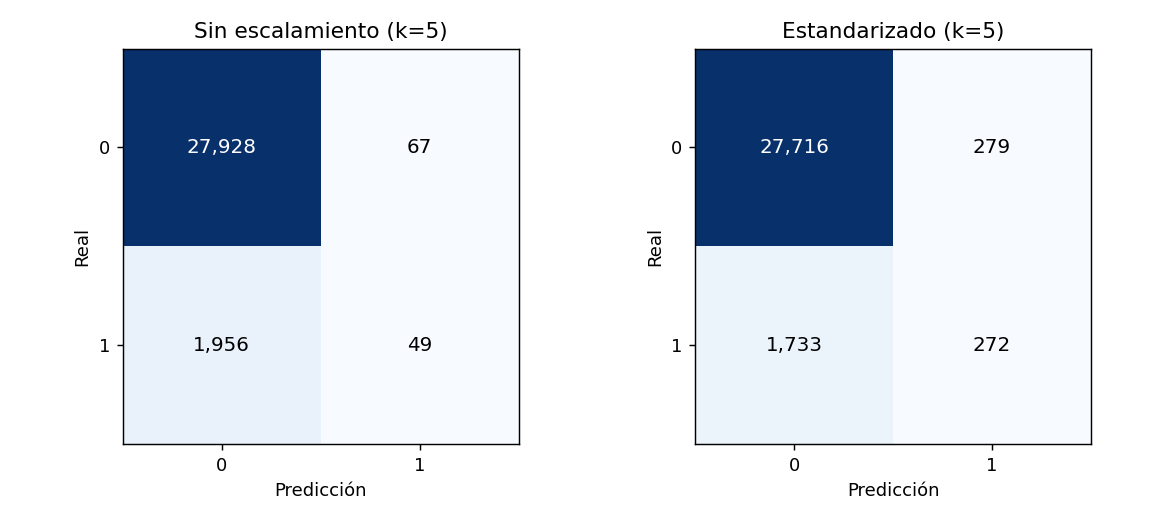
\includegraphics[width=0.85\textwidth]{figuras/ex7_matrices_confusion.png}
    \caption{Matrices de confusión, $k=5$.}
\end{figure}

\begin{enumerate}

\item \textbf{¿Cambió el desempeño tras estandarizar?}
Sí, y de forma sustancial en la capacidad de detectar la clase
positiva: el Accuracy apenas se mueve ($0.9326\to0.9329$), pero el
Recall se multiplica por casi $5.5$ veces ($0.0244\to0.1357$) y el F1
por más de $4.5$ veces ($0.0462\to0.2128$).

\item \textbf{Métrica con el cambio más importante.}
El \textbf{Recall}, y esto es consistente con lo demostrado en el
Ejercicio 3e, pues sin estandarizar las variables como
\texttt{MonthlyIncome} o \texttt{DebtRatio} (con rangos de miles)
dominan el cálculo de distancias por encima de \texttt{age} o
\texttt{NumberOfDependents} (con rangos de decenas o unidades), y el
modelo termina casi ignorando estas últimas, mientras que al
estandarizar todas aportan en una escala comparable y el modelo pasa
de detectar apenas 49 de los 2.005 incumplimientos reales a detectar
272 de esos mismos 2.005.

\item \textbf{Modelo elegido.}
Se recomienda el modelo \textbf{estandarizado}, ya que el Accuracy es
prácticamente igual pero el Recall y el F1 son considerablemente
superiores, y en un problema de riesgo crediticio, donde no detectar
un incumplimiento suele costar más que lanzar una alerta equivocada
(ver Ejercicio 10), esa mejora resulta preferible en casi cualquier
escenario de negocio razonable.

\end{enumerate}
